\documentclass[12pt, a4paper]{article}

\usepackage[utf8]{inputenc}

% Limit the page margin to only 1 inch.
\usepackage[margin=1in]{geometry}

%Imports biblatex package
\usepackage[
backend=biber,
style=alphabetic
]{biblatex}
\addbibresource{../math-342w.bib}

% Enables the `align' environment.
\usepackage{amsmath}
\usepackage{bm}
\usepackage{array}

% Provides useful environments, such as:
% - \begin{proof} ...\end{proof}
\usepackage{amsthm}
\newtheorem{proposition}{Proposition}
\theoremstyle{definition}
\newtheorem*{definition}{Definition}
\newtheorem{theorem}{Theorem}
\newtheorem{corollary}{Corollary}
\newtheorem*{example}{Example}
\newtheorem{algorithm}{Algorithm}

% Enables using \mathbb{}, for example \mathbb{N} for the set of natural numbers.
\usepackage{amssymb}

% Allows using letters in enumerate list environment. Use, for example:
%\begin{enumerate}[label=(\alph*)]
% ...
%\end{enumerate}
\usepackage[inline]{enumitem}

% Enable importing external graphic files and provides useful commands, like \graphicspath{}
\usepackage{graphicx}
% Images are located in a directory called "images" in the current directory.
\graphicspath{{./images/}}

% Make links look better by default.
% See: https://tex.stackexchange.com/questions/823/remove-ugly-borders-around-clickable-cross-references-and-hyperlinks
\usepackage[hidelinks]{hyperref}
\usepackage{xcolor}
\hypersetup{
	colorlinks,
	linkcolor={red!50!black},
	citecolor={blue!50!black},
	urlcolor={blue!80!black}
}

% Code Listings. Source:
% https://stackoverflow.com/questions/3175105/inserting-code-in-this-latex-document-with-indentation
\usepackage{listings}
\usepackage{color}
\usepackage[most]{tcolorbox}

\definecolor{dkgreen}{rgb}{0,0.6,0}
\definecolor{gray}{rgb}{0.5,0.5,0.5}
\definecolor{mauve}{rgb}{0.58,0,0.82}

\lstset{frame=tb,
	language=Java,
	aboveskip=3mm,
	belowskip=3mm,
	showstringspaces=false,
	columns=flexible,
	basicstyle={\small\ttfamily},
	numbers=none,
	numberstyle=\tiny\color{gray},
	keywordstyle=\color{blue},
	commentstyle=\color{dkgreen},
	stringstyle=\color{mauve},
	breaklines=true,
	breakatwhitespace=true,
	tabsize=3
}

\newcommand{\prob}{\text{P}}
%\newcommand{\complement}{\mathsf{c}}
\newcommand{\test}{\text{test}}
\newcommand{\train}{\text{train}}
\newcommand{\select}{\text{select}}
\newcommand{\Dtest}{\mathbb{D}_{\test}}
\newcommand{\Dtrain}{\mathbb{D}_{\train}}
\newcommand{\Dselect}{\mathbb{D}_{\select}}
\title{Lecture 18: MATH 342W: Introduction to Data Science and Machine Learning}
\author{Sergio E. Garcia Tapia\thanks{Based on lectures of Dr. Adam Kapelner at Queens College.
See also the \href{https://github.com/kapelner/QC_MATH_342W_Spring_2025}{course GitHub page}.}}
\date{April 10th, 2025 (last updated \today)}

\begin{document}
	\maketitle
	\section*{R Demo}
	See \verb|QC_MATH_342W_Spring_2025/practice_lectures/lec18.Rmd|.
	\section*{Tree Models}
	Suppose we have a data set $\mathbb{D}$ with a numeric response (output space
	is $\mathcal{Y}=\mathbb{R}$) and one raw feature ($p = 1$), as depicted in 
	Figure~\ref{fig:data-set-numeric-response-1-feature}.
	\begin{figure}
		\centering
		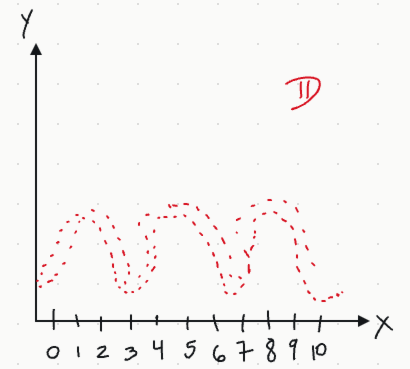
\includegraphics[width=0.3\textwidth]{data-set-numeric-response-1-feature}
		\caption{Data set $\mathbb{D}$ with numeric response space $\mathcal{Y}=\mathbb{R}$
			and 1 feature.}
		\label{fig:data-set-numeric-response-1-feature}
	\end{figure}
	If we wish to make predictions about the phenomenon from which the observations
	in $\mathbb{D}$ were measured, we might first try OLS with a linear fit:
	\begin{align*}
		\mathcal{H}_1 = \{\,
		w_0 + w_1 x \mid \bm{w}\in \mathbb{R}^2
		\,\}
	\end{align*}
	An approximate OLS linear fit $g_1\in \mathcal{H}_1$ is shown in
	Figure~\ref{fig:data-set-numeric-response-1-feature-linear}.
	\begin{figure}
		\centering
		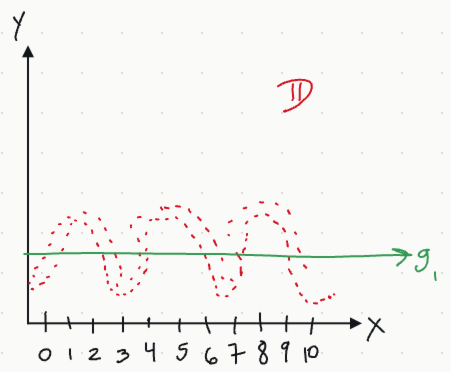
\includegraphics[width=0.3\textwidth]{data-set-numeric-response-1-feature-ols-linear}
		\caption{A linear fit for $\mathbb{D}$ in Figure~\ref{fig:data-set-numeric-response-1-feature}.}
		\label{fig:data-set-numeric-response-1-feature-linear}
	\end{figure}
	By looking at the data set, we can infer that $g_1$ incurs a lot of misspecification
	error since the trend in $\mathbb{D}$ does not appear to be linear.
	Another attempt might be to create a transformed feature $x^2$ and to
	use OLS with a quadratic fit:
	\begin{align*}
		\mathcal{H}_1 = \{\,
		w_0 + w_1 x + w_2 x^2 \mid \bm{w}\in \mathbb{R}^3
		\,\}
	\end{align*}
	An approximate OLS quadratic fit $g_2\in \mathcal{H}_2$ is shown in
	Figure~\ref{fig:data-set-numeric-response-1-feature-quadratic}.
	\begin{figure}
		\centering
		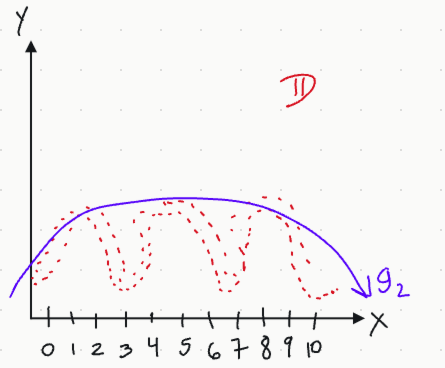
\includegraphics[width=0.3\textwidth]{data-set-numeric-response-1-feature-ols-quadratic}
		\caption{A quadratic fit for $\mathbb{D}$ in Figure~\ref{fig:data-set-numeric-response-1-feature}.}
		\label{fig:data-set-numeric-response-1-feature-quadratic}
	\end{figure}
	The quadratic fit may or may not do any better than the linear fit.
	A third attempt would be to consider a set of candidate functions with sinusoidal
	functions:
	\begin{align*}
		\mathcal{H}_3 = \{\,
		w_0 + w_1 \sin(w_2(x - w_3)) \mid \bm{w}\in \mathbb{R}^4
		\,\}
	\end{align*}
	An approximate least-squares sinusoidal fit $g_3\in \mathcal{H}_3$ is shown in
	Figure~\ref{fig:data-set-numeric-response-1-feature-sine}. We see $g_3$
	likely incurs lower misspecification than $\mathcal{H}_1$ and $\mathcal{H}_2$.
	\begin{figure}
		\centering
		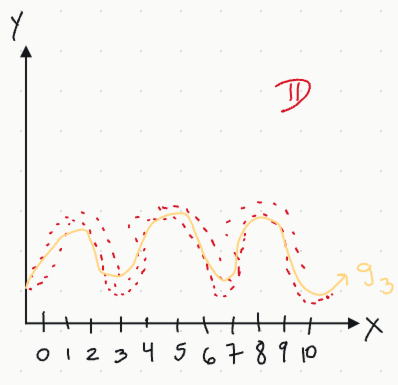
\includegraphics[width=0.3\textwidth]{data-set-numeric-response-1-feature-ols-sine}
		\caption{A sinusoidal fit for $\mathbb{D}$ as from Figure~\ref{fig:data-set-numeric-response-1-feature}.}
		\label{fig:data-set-numeric-response-1-feature-sine}
	\end{figure}
	Note that the least squares fit for $\mathcal{H}_3$ would not be ``ordinary"
	(hence we do not call it OLS), since we cannot create a design matrix $X$
	and compute $(X^\top X)^{-1}X^\top$ to get the least squares best values
	$\bm{w}\in \mathbb{R}^4$. We would need to use an optimizer like \texttt{optimx}
	in R to minimize the objective function
	\begin{align*}
		\sum_{i=1}^{n}(y_i - w_0 + w_1\sin(w_2(x_i-w_3)))^2
	\end{align*}
	
	The point of this exercise was to emphasize that when $p = 1$, the task of
	offering $M$ candidate modeling procedures where at least one performs well
	may be reasonable. However, if $p \gg 1$, how do we offer $M$ such models? We
	lose the ability to visualize, say, 37 dimensions. The problem is that
	\textit{there is no easy way to a priori (before the fact) specify all
	potentially meaningful non-linearities and interactions among features}. This is
	where non-parametric machine learning (hereby abbreviated as ML) comes in.
	
	Note that $\mathcal{H}_1$ has 2 parameters, $\mathcal{H}_2$ has
	3 parameters, and $\mathcal{H}_3$ has 4 parameters.
	By non-parametric, we mean that the number of parameters, and
	the parameter definitions themselves, are \textit{not} pre-specified,
	but they are fit automatically. It is ``as if" the candidate set expands
	to what is needed. We will study \textbf{tree models}. In particular
	\begin{itemize}
		\item \textbf{Regression trees} for when $\mathcal{Y} = \subseteq \mathbb{R}$ (numerical).
		\item \textbf{Classification trees} for when $\mathcal{Y} = \{C_1, \ldots, C_L\}$
		(categorical).
	\end{itemize}
	Both approaches were published in 1984 by Breiman. We are interested in
	the \textbf{Classification and Regression Tree Algorithm (CART)}.
	\section*{Regression Trees}
	For the sake of our discussion, we will continue to consider $\mathcal{Y}=\mathbb{R}$
	and $p=1$ as in Figure~\ref{fig:data-set-numeric-response-1-feature}. Note
	that $x\in \mathcal{X}$, where the input (covariate) space $\mathcal{X} = \mathbb{R}$.
	We can subdivide (partition) it as
	\begin{align*}
		\mathcal{X} = \mathbb{R} =
		\overbrace{(-\infty, 0)}^{A_1} \cup
		\overbrace{[0, 1)}^{A_2} \cup
		\overbrace{[1, 2)}^{A_3} \cup 
		\cdots \cup
		\overbrace{[9, 10)}^{A_{11}} \cup 
		\overbrace{[10, \infty)}^{A_{12}}
	\end{align*}
	Let's transform $x$ from a one-dimensional interval feature to
	a $12$-dimensional categorical variable ($L = 12$), where each category denotes
	membership in one of the sets $A_\ell$. If $X_{\text{raw}}$ is our raw design
	matrix using the raw interval feature $x$, then after the transformation
	we get an $n\times L$ matrix $X$(without intercept):
	\begin{align*}
		X_{\text{raw}}\implies
		X = \begin{bmatrix}
			1 & 0 & \cdots & 0\\
			1 & 0 & \cdots & 0\\
			0 & 1 & \cdots & 0\\
			0 & 1 & \cdots & 0\\
			\vdots& \vdots & \cdots& \vdots\\
			0 & 0 & \cdots& 1\\
			0 & 0 & \cdots & 1
		\end{bmatrix} = \begin{bmatrix}
		\mathbb{I}_{x\in A_1} & \mathbb{I}_{x\in A_2} & \cdots & \mathbb{I}_{x\in A_{12}}
		\end{bmatrix}
	\end{align*}
	Note that if we are assuming that $n \gg p$ and that we have at least one data point in each interval $A_\ell$, $X$ will be full rank. If we fit using OLS, and $x_*$
	is a new observation (in $\mathcal{X}=\mathbb{R}$), our prediction function
	would assign the predicted response $\hat{y}_* = \overline{y}_\ell$ for
	some $\ell$, corresponding to the mean response of the observations in $\mathbb{D}$
	for which $x\in A_\ell$:
	\begin{align*}
		\hat{\bm{y}} = \begin{bmatrix}
			\overline{y}_1\\
			\overline{y}_2\\
			\vdots\\
			\overline{y}_{12}
		\end{bmatrix}
	\end{align*}
	Effectively, we cut the input space into pieces, and we use step functions,
	as depicted in Figure~\ref{fig:data-set-numeric-response-1-feature-step}.
	\begin{figure}
		\centering
		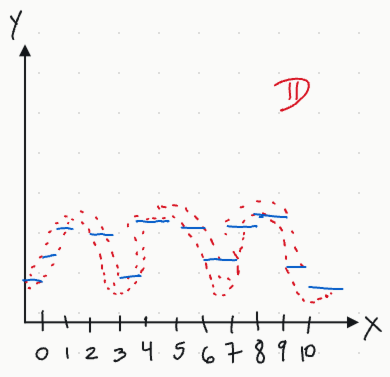
\includegraphics[width=0.35\textwidth]{data-set-numeric-response-1-feature-step}
		\caption{Using step functions to fit the data in
		Figure~\ref{fig:data-set-numeric-response-1-feature}.}
		\label{fig:data-set-numeric-response-1-feature-step}
	\end{figure}
	There is a hyperparameter in this procedure, namely, the size of each interval,
	or equivalently, the number of bins (here 12). This model might not beat
	$\mathcal{H}_3$, but it might do better than $\mathcal{H}_1$ and $\mathcal{H}_2$.
	To select the number of bins, we can use model procedure setting (III) that we discussed
	last lecture. Note that if you use 1 bin, you have the null model $g_0$,
	and if you use $n$ bins (where $n$ is the number of data points), you overfit.
	
	When $p = 1$, there is no much downside to using this approach. What if $p$ is large?
	The Boston Housing data set, for example, has $n = 506$ and $p = 13$. If there
	are 5 bins per feature, then the total number of bins explode exponentially
	to $5^{13}\approx 1.22 \text{ billion}$. We will have many empty bins in this
	case. This is called \textbf{the curse of dimensionality}, i.e., the number
	of parameters grows exponentially with $p$, which is $\gg n$. We will have
	approximately 1.22 billion columns, most consisting only of zeros. In summary,
	this procedure does not extend well to multiple features.
	
	What do we need to do to fix this problem? In our original approach, we carved
	the input space from the get-go into $A_1,A_2,\ldots,A_{12}$. Do we need to do that?
	How about an algorithm $\mathcal{A}$ that dynamically chooses custom bins that
	improve performance? We don't need bins of equal size, or an equal number of bins.
	Figure~\ref{fig:dynamic-split-interval-data} shows an example where $p = 2$.
	\begin{figure}
		\centering
		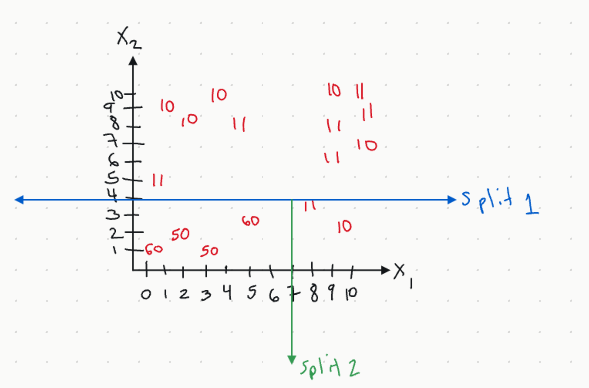
\includegraphics[width=0.5\textwidth]{dynamic-split-interval-data}
		\caption{Dynamically splitting data set with $p = 2$ features.}
		\label{fig:dynamic-split-interval-data}
	\end{figure}
	Let's restrict bins to be orthogonal to the coordinate axes.
	\begin{itemize}
		\item \textbf{Step 1}: Find the best two-bin model by splitting
		all of $\mathbb{R}^2$. In Figure~\ref{fig:dynamic-split-interval-data},
		this was achieved with the line $x_2 = 4$.
		\item \textbf{Step 2}: Find the best three-bin model by
		splitting a previous bin into two bins. In
		Figure~\ref{fig:dynamic-split-interval-data}, this was achieved
		with the line $x_1 = 7$.
		\item \textbf{Step 3}: Find the best four-bin model by splitting a previous
		bin into two bins (not depicted in
		Figure~\ref{fig:dynamic-split-interval-data}).
		\item Eventually, stop.
	\end{itemize}
	Now we can construct a \textbf{rooted binary decision tree} to make predictions, shown in
	Figure~\ref{fig:regression-tree}.
	\begin{figure}
		\centering
		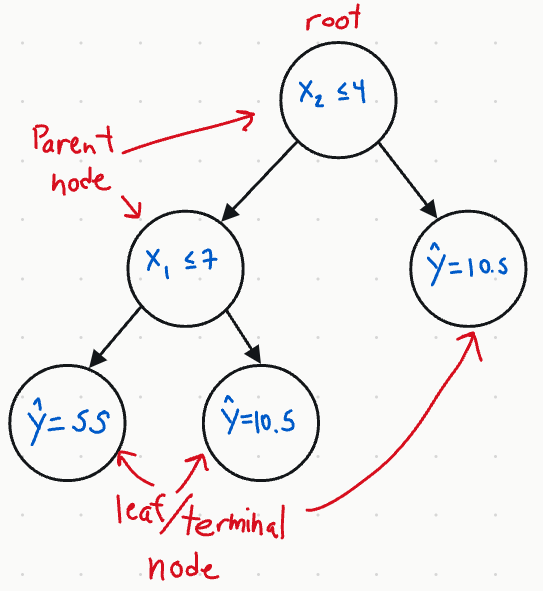
\includegraphics[width=0.4\textwidth]{regression-tree}
		\caption{Binary decision tree built from the partitioning algorithm
		applied in Figure~\ref{fig:dynamic-split-interval-data}.}
		\label{fig:regression-tree}
	\end{figure}
	First, some nomenclature:
	\begin{itemize}
		\item In a rooted tree, there is a node designated as the \textbf{root},
		which is the ancestor of all other nodes. In Figure~\ref{fig:regression-tree},
		it corresponds to the node with $x_2 \leq 4$.
		\item A node may have \textbf{descendants}. A node that has an immediate
		descendant is called a \textbf{parent} node, and its immediate descendants
		are called \textbf{children} nodes.
		\item A node in a tree without any children is called a \textbf{leaf}.
		The leaves in our example correspond to the nodes with $\hat{y}=10.5$, $\hat{y}=55$,
		and $\hat{y}=10.5$.
		\item In a \textbf{binary tree}, each node may have at most 2 children.
	\end{itemize}
	Since we have three bins in our example, there are three values we can predict
	(and hence three leaves in the resulting binary tree). For example,
	if we have an observation with $\bm{x}_* = [x_1 , x_2] = [15, 21]$, then we first
	note $x_2=21$ is larger than $4$, so we immediately predict $\hat{y}_* = 10.5$.
	If instead $\bm{x}_* = [x_1 ,  x_2] = [6 , 2]$, then $x_2\leq 4$ and $x_1\leq 7$,
	so we predict $\hat{y}_* = 55$.
	
	The usage of orthogonal axes in Figure~\ref{fig:dynamic-split-interval-data}
	is depicted by the fact that the lines used to partition the plane are parallel
	to the coordinate axes. Alternatives have been investigated, but it is hard
	to beat random forests and it can be hard to interpret.
	
	Let's state the regression algorithm more fully.
	\begin{tcolorbox}[breakable]
		\begin{algorithm}[Regression Tree Algorithm]
			
			\label{alg:regression-tree-alg}
			Start with $\mathbb{D}$. Let $x_{(i)}$ denote the $i$th smallest
			value in a vector $\bm{u}$.
			\begin{enumerate}[label=(\arabic*)]
				\item Let $\bm{x}_k$ denote the $k$th vector, for $1\leq k\leq p$,
				containing all $n$ possible values for the $k$th feature.
				Let's consider every possible orthogonal-to-axis split, i.e:
				\begin{align*}
					x_1&\leq \bm{x}_{\cdot 1(1)}, x_1 \leq \bm{x}_{\cdot 1(2)}, \ldots, x_1 \leq \bm{x}_{\cdot 1(n-1)}\\
					x_2&\leq \bm{x}_{\cdot 2(1)}, x_2 \leq \bm{x}_{\cdot 2(2)}, \ldots, x_2 \leq \bm{x}_{\cdot 2(n-1)}\\
					\vdots &\leq  \vdots \\
					x_p&\leq \bm{x}_{\cdot p(1)}, x_p \leq \bm{x}_{\cdot p(2)}, \ldots, x_p \leq \bm{x}_{\cdot p(n-1)}\\
				\end{align*}
				This means we have $n\cdot (p-1)$ possible splits. Note we do not
				consider, for example, $x_1\leq \bm{x}_{\cdot 1(n)}$,
				or $x_2\leq \bm{x}_{\cdot 2(n)}$, and so on because such a split
				would have \textit{all} data on one side of the split, and hence
				there is no split at all.
				\item Pick the best split, i.e., the one with the lowest error,
				where error is defined as:
				\begin{align*}
					SSE_{\text{weighted}} := \frac{n_L SSE_L + n_R SSE_R}{n_L + n_R}
				\end{align*}
				where $n_L$ is the number of observations in the left child,
				$n_R$ is the number of observations in the right child, $SSE_L$
				is the $SSE$ in the left child, and $SSR_R$ is the $SSE$ in
				the right child. Note that since we are fitting a local
				optimization by picking the \textit{best} split each time, this
				algorithm $\mathcal{A}$ is \textit{greedy}.
				\item Repeat steps (1) and (2) on the subset of $\mathbb{D}$
				consisting of all the daughter nodes. Note that we can make
				at most $n$ splits, otherwise we will have $n$ dummies and we
				would surely overfit. Therefore, stop when the number of points
				in a child node is below some threshold $N_0$ (default $N_0 = 5$).
			\end{enumerate}
		\end{algorithm}
	\end{tcolorbox}
	\section*{Classification Trees}
	Let $\mathcal{Y} = \{C_1, \ldots, C_L\}$ (categorical response space).
	The classification tree algorithm is similar to Algorithm~\ref{alg:regression-tree-alg},
	but differs a bit in steps 2 and 3.
	
	\begin{tcolorbox}[breakable]
		\begin{algorithm}[Classification Tree Algorithm]\label{alg:classification-tree-alg}
			Start with $\mathbb{D}$. Let $x_{(i)}$ denote the $i$th smallest
			value in a vector $\bm{u}$.
			\begin{enumerate}[label=(\arabic*)]
				\item Let $\bm{x}_k$ denote the $k$th vector, for $1\leq k\leq p$,
				containing all $n$ possible values for the $k$th feature.
				Let's consider every possible orthogonal-to-axis split, i.e:
				\begin{align*}
					x_1&\leq \bm{x}_{\cdot 1(1)}, x_1 \leq \bm{x}_{\cdot 1(2)}, \ldots, x_1 \leq \bm{x}_{\cdot 1(n-1)}\\
					x_2&\leq \bm{x}_{\cdot 2(1)}, x_2 \leq \bm{x}_{\cdot 2(2)}, \ldots, x_2 \leq \bm{x}_{\cdot 2(n-1)}\\
					\vdots & \leq  \vdots\\
					x_p&\leq \bm{x}_{\cdot p(1)}, x_p \leq \bm{x}_{\cdot p(2)}, \ldots, x_p \leq \bm{x}_{\cdot p(n-1)}\\
				\end{align*}
				This means we have $n\cdot (p-1)$ possible splits. Note we do not
				consider, for example, $x_1\leq \bm{x}_{\cdot 1(n)}$,
				or $x_2\leq \bm{x}_{\cdot 2(n)}$, and so on because such a split
				would have \textit{all} data on one side of the split, and hence
				there is no split at all.
				\item Pick the best split, i.e., the one with the lowest error.
				We need a new error metric because $SSE$ is not appropriate for
				a categorical response. Define the \textbf{Gini} error metric:
				\begin{align*}
					G_{\text{neighbor, avg}} = \frac{n_L G_L + n_R G_R}{n_L + n_R}
				\end{align*}
				where $n_L$ is the number of observations in the left child,
				and $n_R$ is the number of observations in the right child.
				We get something similar to $SSE$ by defining
				\begin{align*}
					G := \sum_{\ell=1}^{\text{num levels}}\hat{p}_\ell(1 - \hat{p}_\ell)
				\end{align*}
				where $\hat{p}_\ell$ is the proportion of observations whose response
				is category $\ell$ in a given node:
				\begin{align*}
					\hat{p}_\ell := \frac{
						\text{number of observations with category $\ell$ in node}}
					{\text{total number of observations in node}}
				\end{align*}
				Note that since we fitting a local optimization by picking
				the \textit{best} split each time, this algorithm $\mathcal{A}$ 
				is \textit{greedy}.
				\item Repeat steps (1) and (2) on the subset of $\mathbb{D}$
				consisting of all the daughter nodes. Note that we can make
				at most $n$ splits, otherwise we will have $n$ dummies and we
				would surely overfit. Therefore, stop when the number of points
				in a child node is below some threshold (default $N_0=1$,
				possibly because there are only $L$ levels).
			\end{enumerate}
		\end{algorithm}
	\end{tcolorbox}
	See Figure~\ref{fig:dynamic-split-categorical-data} and
	Figure~\ref{fig:classification-tree} for an example of applying
	Algorithm~\ref{alg:classification-tree-alg}.
	\begin{figure}
		\centering
		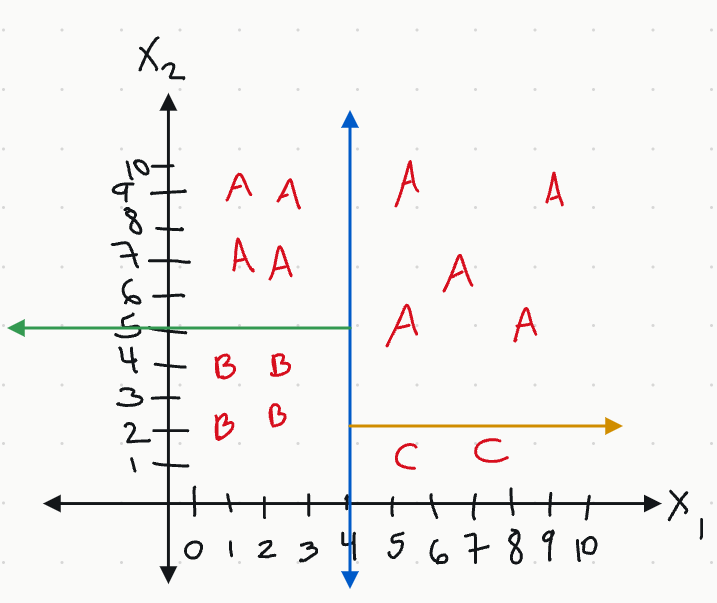
\includegraphics[width=0.4\textwidth]{dynamic-split-categorical-data}
		\caption{Classification tree algorithm with a categorical response space.}
		\label{fig:dynamic-split-categorical-data}
	\end{figure}
	\begin{figure}
		\centering
		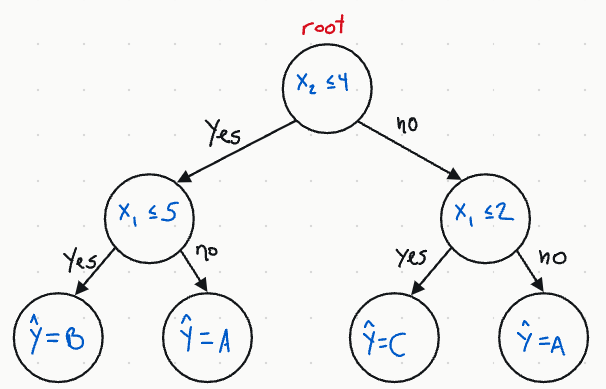
\includegraphics[width=0.5\textwidth]{classification-tree}
		\caption{Classification tree corresponding to
			Figure~\ref{fig:dynamic-split-categorical-data}.}
		\label{fig:classification-tree}
	\end{figure}
	The larger $G$ is, the more heterogeneous the node is. For example, if the
	node has all $A$'s, then $\hat{p}_A = \hat{p}_B = \hat{p}_C = 0$, and
	hence $G=0$ for that node.
	\pagebreak
	\printbibliography
\end{document}